\documentclass[a4paper,14pt]{extbook}
\usepackage[utf8]{inputenc}
\usepackage{hyperref}
\hypersetup{
    colorlinks=true,
    linkcolor=blue,
    filecolor=magenta,      
    urlcolor=cyan,
}
\usepackage{graphicx}
\graphicspath{ {./images/} }
\usepackage[legalpaper, margin=0.70in]{geometry}
\usepackage{listings}

\title{Akarin Engine}
\author{Hanif Bin Ariffin}

\begin{document}

\maketitle
\tableofcontents

\newpage
\section{Introduction}

A \href{https://www.youtube.com/watch?v=BbLW4ZJnaLM}{demo} of some version of the engine.

This project was supposed to be a simple calculator.
Somehow, it became a freak-of-nature ala Frankenstein of an attempt at making a 3d engine.
My current goal is to be able to implement all kinds of rendering techniques (mostly lighting, shadows, etc etc).

After that, I might implement other stuff like physics, animation, sounds, scripts etc. etc. for it to become a proper game engine.

Many terminologies will be used in this book without regard to its proper usage.
I am bad at this, so if you find me using inaccurate word to describe things then feel free to comment.

\newpage
\section{Motivation}

\begin{figure}[h]
    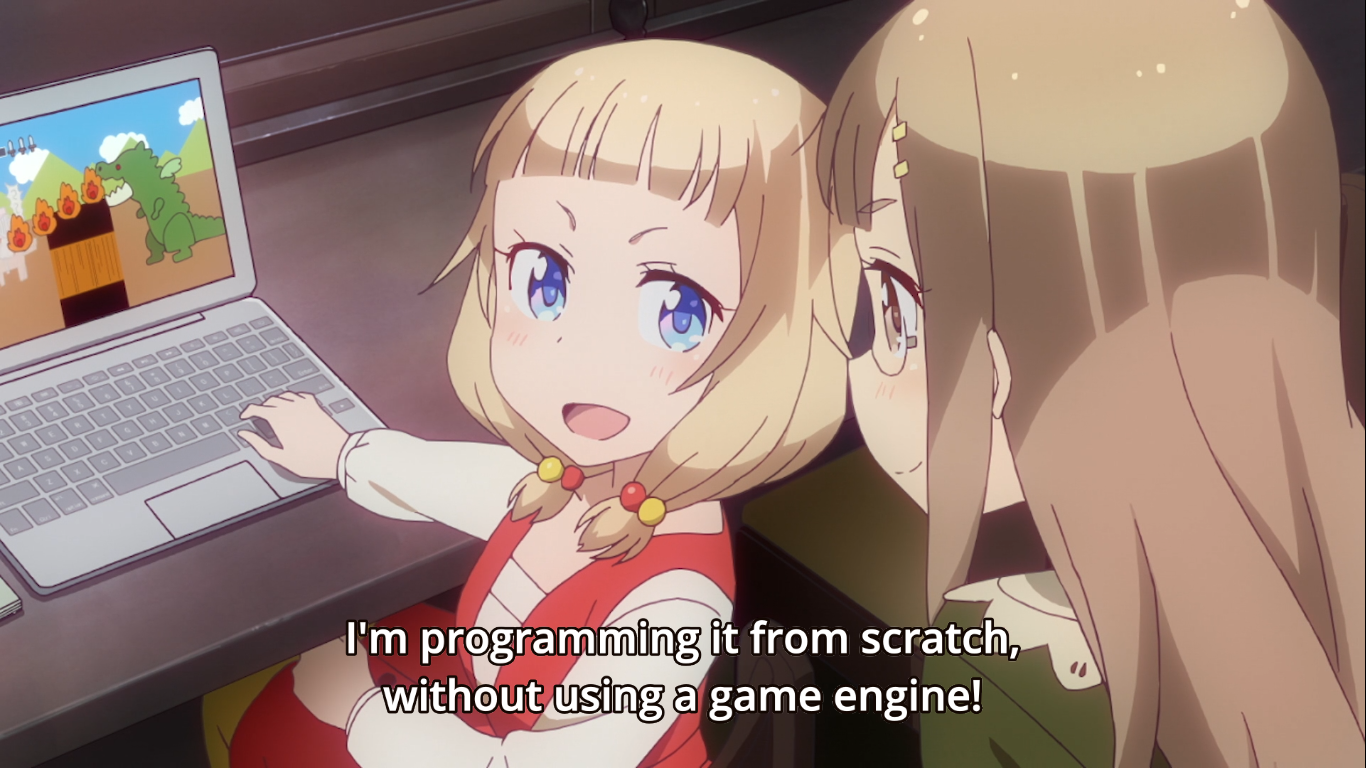
\includegraphics[width=\textwidth]{.images/nenechi_writes_game_engine.png}
    \caption{If Nenecchi from \textit{New Game!!} can write a game engine from scratch by herself, what's stopping you?}
\end{figure}

Honestly, this engine does not have a specific motivation.
It is an amalgamation of several sparks of interest that lead me to writing it.

First, while I was contributing to Godot Engine I realize how hard it is to manage large codebases.
Upon reading Data-Oriented Design by Richard Fabian, I see why using OOP doesn't help when maintaining an ever growing project.
If you want to know why, just read the book.
The first few chapters are especially instructive to software architecture in general while the later chapters tackle game engine architecture specifically.

Second, I am interested 3D graphics in general.
Whenever I play games, I will always think of how they do it, and how I would (hypothetically) do them myself.
However, without any knowledge of writing 3d renderer I didn't have anything to look forward to.
That is until I decided to start picking up \href{https://www.amazon.ca/Game-Engine-Architecture-Jason-Gregory/dp/1568814135}{Game Engine Architecture}, \href{https://www.cs.utexas.edu/users/fussell/courses/cs354/handouts/Addison.Wesley.OpenGL.Programming.Guide.8th.Edition.Mar.2013.ISBN.0321773039.pdf}{OpenGL Redbook} and \href{https://learnopengl.com}{LearnOpenGL}

Thus, this project can be thought of as my feeble attempt at implementing what I have learnt so far.
Therefore, any decisions made in this project \textit{is going to be dumb}.
As such, any comments, criticisms, and suggestions are always helpful.

\newpage
\section{Installation}

Please head over to the README file \href{run:./../README.md}{here}.

\newpage
\section{Basic OpenGL}

This project uses OpenGL to perform many tasks required to render a frame.

\section{Appendices}

\end{document}
